\section{نتیجه گیری}
\label{s:conclusion}
با بررسی ها و مرور پژوهش‌های انجام شده در این مطالعه می‌توان روی آوردن محققان به سمت داده‌های چشمی را به دلالیل عنوان شده در زیربخش
\ref{ss:ProVsCon}
را مشاهده نمود. از طرفی دستگاه‌ها و سیستم‌های جدید کامپیوتری که انسان در جنبه‌های مختلف زندگی با آن‌ها در ارتباط است به سمت کم حجم شدن و راحتی کاربر می‌روند و یکی از راه‌های ارتباطی چشم انسان است، که می‌تواند داده های بسیار خوبی حتی به صورت هم‌زمان از وضعیت شناختی کاربر بدهد، و این در حالی است که نیازی به دستگاه اضافی و یا مکان خاص نمی‌باشد.
\\
به نظر می‌رسد در صورت انتخاب درست ویژگی‌ها و مشخصه‌های آن  و ترکیب وزن‌دار و یا معمولی آن‌ها می‌توان با دقت خوبی حتی به صورت همزمان وضعیت شناختی کاربر را گزارش نمود.
در شکل
\ref{fig:eyetree}
می‌توانید نمودار درختی انواع داده های چشمی و مشخصه هر کدام را ببینید که تعدادی از آنها به طور کامل در زیربخش
\ref{ss:EyeMeasure}
بررسی شد را ببینید.

\begin{figure}[htbp]
	\centering
	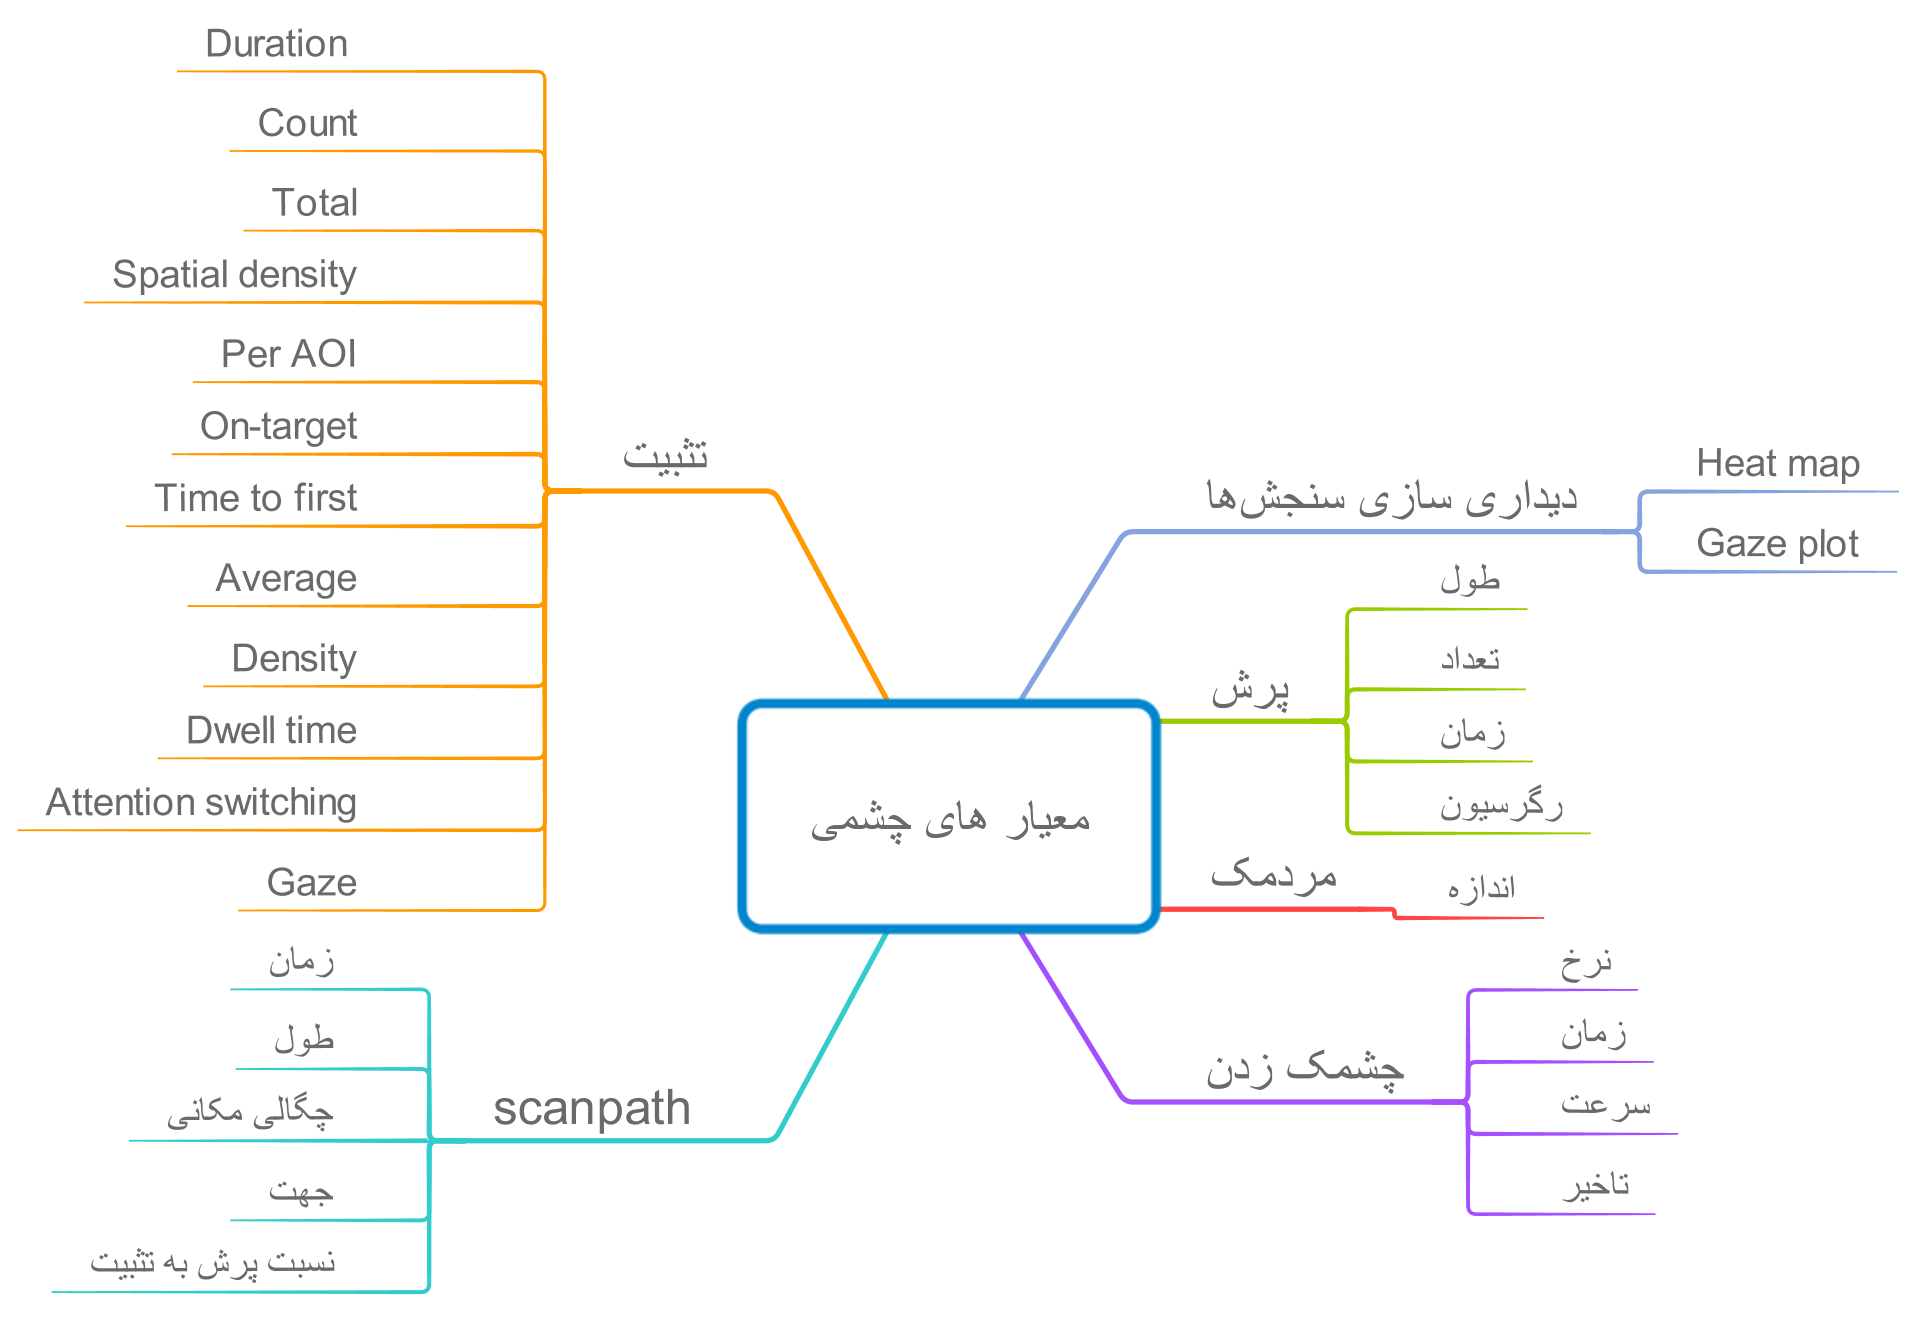
\includegraphics[width=\linewidth]{figures/eye_tree}
	\caption[نمودار درختی داده‌های چشمی]{نمودار درختی انواع داده‌های چشمی و مشخصه هرکدام}
	\label{fig:eyetree}
\end{figure}
جاکوب و همکاران
\cite{Hyona2003}
در پژوهش مروری که انجام دادند میزان استفاده از هریک از داده‌های چشمی در سنجش بار شناختی را گزارش کردند.
در شکل 
\ref{fig:eyedataused}
حاصل گزارش آن‌ها را مشاهده می‌کنید.
\begin{figure}[htbp]
	\centering
	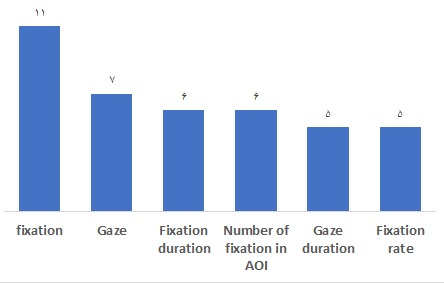
\includegraphics[width=0.7\linewidth]{figures/eyedata_used}
	\caption[میزان استفاده از داده‌های چشمی]{نمودار میزان استفاده از هر یک از داده‌های چشمی}
	\label{fig:eyedataused}
\end{figure}
